% \iffalse meta-comment
%
% Copyright (C) 2015 by Matthew Wardrop <mister.wardrop@gmail.com>
% ---------------------------------------------------------------------------
% This work may be distributed and/or modified under the
% conditions of the LaTeX Project Public License, either version 1.3
% of this license or (at your option) any later version.
% The latest version of this license is in
%   http://www.latex-project.org/lppl.txt
% and version 1.3 or later is part of all distributions of LaTeX
% version 2005/12/01 or later.
%
% This work has the LPPL maintenance status `maintained'.
%
% The Current Maintainer of this work is Matthew Wardrop
%
% This work consists of the files blochsphere.dtx and blochsphere.ins
% and the derived filebase blochsphere.sty.
%
% \fi
%
% \iffalse
%<*driver>
\ProvidesFile{blochsphere.dtx}
%</driver>
%<package>\NeedsTeXFormat{LaTeX2e}[1999/12/01]
%<package>\ProvidesPackage{blochsphere}
%<*package>
    [2015/08/17 v1.0 blochsphere drawing package]
%</package>
%
%<*driver>
\documentclass{ltxdoc}
\EnableCrossrefs
\CodelineIndex
\RecordChanges
\usepackage{blochsphere}
\usepackage{minted}
\usepackage{hyperref}

\setlength{\parskip}{0.7em}

\newenvironment{key}[2]{
	\noindent{\llap{Option: \bf\tt #2\hskip 9pt}}
}{}
\newcommand{\DescribeKey}[3][]{
	\noindent{\llap{\bf\tt #2\hskip 9pt}[default = #1] #3}
}

\usepackage{listings}
\lstset{breaklines=true}

\begin{document}
  \DocInput{blochsphere.dtx}
  \PrintChanges
  \PrintIndex
\end{document}
%</driver>
% \fi
%
% \CheckSum{0}
%
% \CharacterTable
%  {Upper-case    \A\B\C\D\E\F\G\H\I\J\K\L\M\N\O\P\Q\R\S\T\U\V\W\X\Y\Z
%   Lower-case    \a\b\c\d\e\f\g\h\i\j\k\l\m\n\o\p\q\r\s\t\u\v\w\x\y\z
%   Digits        \0\1\2\3\4\5\6\7\8\9
%   Exclamation   \!     Double quote  \"     Hash (number) \#
%   Dollar        \$     Percent       \%     Ampersand     \&
%   Acute accent  \'     Left paren    \(     Right paren   \)
%   Asterisk      \*     Plus          \+     Comma         \,
%   Minus         \-     Point         \.     Solidus       \/
%   Colon         \:     Semicolon     \;     Less than     \<
%   Equals        \=     Greater than  \>     Question mark \?
%   Commercial at \@     Left bracket  \[     Backslash     \\
%   Right bracket \]     Circumflex    \^     Underscore    \_
%   Grave accent  \`     Left brace    \{     Vertical bar  \|
%   Right brace   \}     Tilde         \~}
%
%
% \changes{v1.0}{2015/08/17}{Initial version}
%
% \DoNotIndex{\newcommand,\newenvironment}
%
% \providecommand*{\url}{\texttt}
% \GetFileInfo{blochsphere.dtx}
% \title{The \textsf{blochsphere} package}
% \author{Matthew Wardrop \\ \url{mister.wardrop@gmail.com}}
% \date{\fileversion~from \filedate}
%
% \maketitle
%
% \tableofcontents
%
% \section{Introduction}
%
% The |blochsphere| package is used to draw pseudo-3D Blochsphere diagrams, such as that
% shown in figure \ref{fig:blochsphere}. It supports various annotations, such as
% great and small circles, axes, rotation markings and state vectors. It can be used
% in a standalone fashion, or nested within a |tikzpicture| environment by setting
% the environment option |nested| to |true|.
%
% \section{Usage}
%
% Using |blochsphere| is as simple as creating a `blochsphere' environment.
% \begin{minted}{LaTeX}
% \begin{blochsphere}[<options>]
% ...
% \end{blochsphere}
% \end{minted}
% By default, this will create a blank Bloch sphere ready for annotation. The options can be
% any of those described in the next section.
%
% \noindent\DescribeMacro{\drawBall} \oarg{options}\\
% This macro draws the basic Bloch sphere, according to the options defined in the next section.
%
% \noindent\DescribeMacro{\drawBallGrid} \oarg{options} \marg{latdegsep} \marg{longdegsep}\\
% This macro draws latitude and longitude circles at an interval defined by |latdegsep| and |longdegsep| respectively.
%
% \noindent\DescribeMacro{\setDrawingPlane} \oarg{options} \marg{tiltangle} \marg{rotationangle}\\
% This macro defines a transformation matrix within TikZ to create the effect of 2D projections of 3D planes,
% named according to the |plane| option. This is used internally in all of the drawing commands.
%
% \noindent\DescribeMacro{\setLatitudinalDrawingPlane} \oarg{options} \marg{latitude}\\
% This is a special case of |\setDrawingPlane| that constructs the transform required to draw a 2D image in
% a latitudinal plane.
%
% \noindent\DescribeMacro{\setLongitudinalDrawingPlane} \oarg{options} \marg{longitude}\\
% This is a special case of |\setDrawingPlane| that constructs the transform required to draw a 2D image in
% a longitudinal plane.
%
% \noindent\DescribeMacro{\drawCircle} \oarg{options} \marg{tiltangle} \marg{rotationangle}\\
% Draws a circle on the surface of a Bloch sphere around the axis which is tilted by |tiltangle|
% from the z-axis and with a rotation of |rotationangle| about the z-axis.
%
% \noindent\DescribeMacro{\drawGreatCircle} \oarg{options} \marg{tiltangle} \marg{rotationangle}\\
% An alias of |\drawCircle|.
%
% \noindent\DescribeMacro{\drawSmallCircle} \oarg{options} \marg{tiltangle} \marg{rotationangle} \marg{offsetLatitude}\\
% Draws a circle on the surface of a Bloch sphere around the axis which is tilted by |tiltangle|
% from the z-axis and with a rotation of |rotationangle| about the z-axis, with an offset along the axis
% such that it reaches an effective latitude of |offsetLatitude|.
%
% \noindent\DescribeMacro{\drawLatitudeCircle} \oarg{options} \marg{latitude}\\
% Draws a circle on the Bloch sphere corresponding to the given latitude.
%
% \noindent\DescribeMacro{\drawLongitudeCircle} \oarg{options} \marg{longitude}\\
% Draws a great circle on the Bloch sphere corresponding to the given longitude.
%
% \noindent\DescribeMacro{\drawRotationLeft} \oarg{options} \marg{tiltangle} \marg{rotationangle} \marg{axisoffset} \marg{clearangle}\\
% Draw a left-handed rotation about the Bloch sphere, titled and rotated as for a circle
% with the same parameters, with a gap in the line where the arrow should go of
% |clearangle| degrees.
%
% \noindent\DescribeMacro{\drawRotationRight} \oarg{options} \marg{tiltangle} \marg{rotationangle} \marg{axisoffset} \marg{clearangle}\\
% As above, but a right-handed rotation annotation.
%
% \noindent\DescribeMacro{\drawAxis} \oarg{options} \marg{tiltangle} \marg{rotationangle}\\
% Draw a line along the axis tilted |tiltangle| degrees from the z-axis, rotated about
% the z-axis by |rotationangle| degrees.
%
% \noindent\DescribeMacro{\labelPolar} \oarg{options} \marg{tikzlabel} \marg{tiltangle} \marg{rotationangle}\\
% Assign a tikz label to the point identified by an angle |tiltangle| from the z-axis
% and a rotation |rotationangle| about the z-axis.
%
% \noindent\DescribeMacro{\labelLatLon} \oarg{options} \marg{tikzlabel} \marg{latitude} \marg{longitude}\\
% Assign a tikz label to the point identified the specified latitude and longitude.
%
% \noindent\DescribeMacro{\drawStatePolar} \oarg{options} \marg{tikzlabel} \marg{tiltangle} \marg{rotationangle}\\
% Draw a vector from the origin to the point identified by an angle |tiltangle|
% from the z-axis and a rotation |rotationangle| about the z-axis, which will
% be labelled |tikzlabel|.
%
% \noindent\DescribeMacro{\drawStateLatLon} \oarg{options} \marg{tikzlabel} \marg{latitude} \marg{longitude}\\
% Draw a vector from the origin to the point identified by the provided
% latitude and longitude, which will be labelled |tikzlabel|.
%
%
% \section{Package, Environment and Macro options}
% For convenience, all options at all levels share the same namespace. Therefore, all
% options passed to the package will be the defaults for all environment, which will
% in turn be the defaults for all subsequent macro calls.
%
%
% \DescribeKey[1.5cm]{radius}
% {This option controls the radius of the qubit, and can be specified in any valid \LaTeX units.}
%
%
% \DescribeKey[15]{tilt}{This option controls the tilt (into the page) of the top of the bloch sphere (in degrees).}
%
%
% \DescribeKey[-20]{rotation}{This option controls the (right-handed) rotation of the Blochsphere around the (potentially tilted) z-axis, also specified in degrees.}
%
%
% \DescribeKey[white]{color}{This specifies the colour of the drawn ball.}
%
%
% \DescribeKey[0.7]{opacity}{This option controls the opacity of the ball, allowing lines drawn behind the ball to be visible.}
%
%
% \DescribeKey[]{style}{This option controls the current drawing style, and supports any valid tikz styling.}
%
%
% \DescribeKey[1]{scale}{This option allows one to temporarily change the scale of drawn circles/etc, allowing annotations to ``hover'' over the Bloch sphere.}
%
%
% \DescribeKey[current plane]{plane}{The name which should label the current plane being defined, or the plane to be used.}
%
%
% \DescribeKey[(0,0,0)]{shift}{The three dimensional offset by which the currently being drawn objects should be shifted.}
%
%
% \DescribeKey[3d]{ball}{Specifies how the ball should be drawn. Options are: {\tt 3d}, {\tt circle}, {\tt none}}
%
%
% \DescribeKey[black]{statecolor}{The color with which the state vectors should be drawn.}
%
%
% \DescribeKey[0.4pt]{statewidth}{The width with which state vectors should be drawn.}
%
%
% \DescribeKey[]{axisarrow}{The arrow to use at the end of a drawn axis.}
%
%
% \DescribeKey[false]{labelmark}{Whether a black dot should be drawn at the point being labelled.}
%
%
% \DescribeKey[false]{nested}{Whether the {\tt blochsphere} environment is being nested in a |tikzpicture| environment. If it is nested, then this should be set to true.}
%
%
% \section{Example}
% In this section we provide example code to generate the following diagram:
%
% \begin{figure}[h!]
% \begin{center}
% 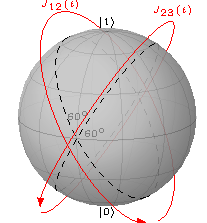
\includegraphics{example.pdf}
% \end{center}
% \caption{Example Bloch Sphere \label{fig:blochsphere}}
% \end{figure}
%
% \newminted{latex}{gobble=2,linenos}
% \begin{latexcode}
% \begin{blochsphere}[radius=1.5 cm,tilt=15,rotation=-20]
%     \drawBallGrid[style={opacity=0.3}]{30}{30}
%
%     \drawGreatCircle[style={dashed}]{-60}{0}{0}
%     \drawGreatCircle[style={dashed}]{60}{0}{0}
%
%     \drawRotationLeft[scale=1.3,style={red}]{-60}{0}{0}{15}
%     \drawRotationRight[scale=1.3,style={red}]{60}{0}{0}{15}
%
%     \node at (-0.8,1.9) {\textcolor{red}{\tiny $J_{12}(t)$}};
%     \node at (1.1,1.8) {\textcolor{red}{\tiny $J_{23}(t)$}};
%
%     \labelLatLon{up}{90}{0};
%     \labelLatLon{down}{-90}{90};
%     \node[above] at (up) {{\tiny $\left|1\right>$ }};
%     \node[below] at (down) {{\tiny $\left|0\right>$}};
%
%     \labelLatLon[labelmark=false]{d}{15}{90};
%     \node at (d) {\color{gray}\fontsize{0.15cm}{1em}\selectfont $60^\circ$};
%
%     \labelLatLon[labelmark=falsa]{d2}{5}{78};
%     \node at (d2) {\color{gray}\fontsize{0.15cm}{1em}\selectfont $60^\circ$};
% \end{blochsphere}
% \end{latexcode}
%
% \StopEventually{}
%
% \section{Implementation}
%
% \iffalse
%<*package>
% \fi
% \subsection{Preamble}
%    \begin{macrocode}
\NeedsTeXFormat{LaTeX2e}[1994/06/01]
\ProvidesPackage{blochsphere}[2015/08/17]
%    \end{macrocode}
% \iffalse
%% \usepackage{trace}
%%\tracingall
% \fi
%
%    \begin{macrocode}
\usepackage{tikz,etoolbox,environ,ifthen,kvsetkeys,kvoptions}
\usetikzlibrary{decorations.pathreplacing, decorations.markings, calc, fadings}
%    \end{macrocode}
%
% \subsection{Package/Environment/Macro options}
%
% \begin{key}{blochsphere}{radius}
%    \begin{macrocode}
\define@key{blochsphere}{radius}{%
	\def\blochsphere@radius{#1}%
}
\providecommand{\blochsphere@radius}{1cm}
%    \end{macrocode}
% \end{key}
%
%
% \begin{key}{blochsphere}{tilt}
%    \begin{macrocode}
\define@key{blochsphere}{tilt}{%
	\def\blochsphere@tilt{#1}%
}
\providecommand{\blochsphere@tilt}{15}
%    \end{macrocode}
% \end{key}
%
%
% \begin{key}{blochsphere}{rotation}
%    \begin{macrocode}
\define@key{blochsphere}{rotation}{%
	\def\blochsphere@rotation{#1}%
}
\providecommand{\blochsphere@rotation}{-20}
%    \end{macrocode}
% \end{key}
%
%
% \begin{key}{blochsphere}{color}
%    \begin{macrocode}
\define@key{blochsphere}{color}{%
	\def\blochsphere@color{#1}%
}
\providecommand{\blochsphere@color}{white}
%    \end{macrocode}
% \end{key}
%
%
% \begin{key}{blochsphere}{opacity}
%    \begin{macrocode}
\define@key{blochsphere}{opacity}{%
	\def\blochsphere@opacity{#1}%
}
\providecommand{\blochsphere@opacity}{0.7}
%    \end{macrocode}
% \end{key}
%
%
% \begin{key}{blochsphere}{style}
%    \begin{macrocode}
\define@key{blochsphere}{style}{%
	\def\blochsphere@style{#1}%
}
\providecommand{\blochsphere@style}{}
%    \end{macrocode}
% \end{key}
%
%
% \begin{key}{blochsphere}{scale}
%    \begin{macrocode}
\define@key{blochsphere}{scale}{%
	\def\blochsphere@scale{#1}%
}
\providecommand{\blochsphere@scale}{1}
%    \end{macrocode}
% \end{key}
%
%
% \begin{key}{blochsphere}{plane}
%    \begin{macrocode}
\define@key{blochsphere}{plane}{%
	\def\blochsphere@plane{#1}%
}
\providecommand{\blochsphere@plane}{current plane}
%    \end{macrocode}
% \end{key}
%
%
% \begin{key}{blochsphere}{shift}
%    \begin{macrocode}
\define@key{blochsphere}{shift}{%
	\def\blochsphere@shift{{#1}}%
}
\providecommand{\blochsphere@shift}{{0,0,0}}
%    \end{macrocode}
% \end{key}
%
%
% \begin{key}{blochsphere}{ball}
%    \begin{macrocode}
\define@key{blochsphere}{ball}{%
	\def\blochsphere@ball{#1}%
}
\providecommand{\blochsphere@ball}{3d}
%    \end{macrocode}
% \end{key}
%
%
% \begin{key}{blochsphere}{statecolor}
%    \begin{macrocode}
\define@key{blochsphere}{statecolor}{%
	\def\blochsphere@statecolor{#1}%
}
\providecommand{\blochsphere@statecolor}{black}
%    \end{macrocode}
% \end{key}
%
%
% \begin{key}{blochsphere}{statewidth}
%    \begin{macrocode}
\define@key{blochsphere}{statewidth}{%
	\def\blochsphere@statewidth{#1}%
}
\providecommand{\blochsphere@statewidth}{0.4pt}
%    \end{macrocode}
% \end{key}
%
%
% \begin{key}{blochsphere}{axisarrow}
%    \begin{macrocode}
\define@key{blochsphere}{axisarrow}{%
	\def\blochsphere@axisarrow{#1}%
}
\providecommand{\blochsphere@axisarrow}{}
%    \end{macrocode}
% \end{key}
%
%
% \begin{key}{blochsphere}{labelmark}
%    \begin{macrocode}
\define@key{blochsphere}{labelmark}{%
    \setboolean{blochsphere@labelmark}{#1}%
}
\newboolean{blochsphere@labelmark}
\setboolean{blochsphere@labelmark}{false}
%    \end{macrocode}
% \end{key}
%
%
% \begin{key}{blochsphere}{nested}
%    \begin{macrocode}
\define@key{blochsphere}{nested}{%
	\setboolean{blochsphere@nested}{#1}%
}
\newboolean{blochsphere@nested}
\setboolean{blochsphere@nested}{false}
%    \end{macrocode}
% \end{key}
%	\begin{macrocode}
\ProcessKeyvalOptions{blochsphere}\relax
%    \end{macrocode}
%
% \subsection{{\bfseries\tt blochsphere} Environment}
%	 This is the central environment definition. Note that all macros defined
%	 below will only be defined within this environment.
%
% \begin{environment}{blochsphere}
%    \begin{macrocode}
\newenvironment{blochsphere}[1][]{
	\begingroup
	\makeatletter
	\ignorespaces\setkeys{blochsphere}{#1}\unskip%
	\pgfdeclarelayer{back}%
	\pgfdeclarelayer{front}%
	\pgfsetlayers{back,main,front}%
	\pgfkeys{%
		/tikz/on layer/.code={%
			\pgfonlayer{##1}\begingroup%
			\aftergroup\endpgfonlayer%
			\aftergroup\endgroup%
		},%
		/tikz/node on layer/.code={%
			\gdef\node@@on@layer{%
			\setbox\tikz@tempbox=\hbox\bgroup\pgfonlayer{##1}\unhbox\tikz@tempbox\endpgfonlayer\egroup}%
			\aftergroup\node@on@layer%
		},%
		/tikz/end node on layer/.code={%
			\endpgfonlayer\endgroup\endgroup%
		}%
	}%
	\def\node@on@layer{\aftergroup\node@@on@layer}%
%    \end{macrocode}
%    \begin{macro}{\drawBall}
%        \begin{macrocode}
	\newcommand\drawBall[1][]{
	\begingroup
		\setkeys{blochsphere}{##1}
		\expandafter\ifstrequal\expandafter{\blochsphere@ball}{3d}{
			\fill[on layer=main,ball color=\blochsphere@color,opacity=\blochsphere@opacity] (0,0) circle (\blochsphere@radius); % 3D lighting effect
		}{}
		\expandafter\ifstrequal\expandafter{\blochsphere@ball}{circle}{
			\draw[on layer=main,color=\blochsphere@color] (0,0) circle (\blochsphere@radius); % 3D lighting effect
		}{}
	\endgroup
	}%
%    \end{macrocode}
%    \end{macro}
%    \begin{macro}{\drawBallGrid}
%        \begin{macrocode}
	\newcommand\drawBallGrid[3][]{
	\begingroup
		\setkeys{blochsphere}{##1}
		\foreach \phi in {0,##2,...,89} {
			\drawLatitudeCircle{\phi}
			\drawLatitudeCircle{-\phi}
		}
		\foreach \theta in {0,##3,...,179} {
			\drawLongitudeCircle{\theta}
		}
	\endgroup
	}%
%    \end{macrocode}
%    \end{macro}
%    \begin{macro}{\setDrawingPlane}
%        \begin{macrocode}
	\newcommand\setDrawingPlane[3][]{%
		\setkeys{blochsphere}{##1}
		\pgfmathsetmacro\aphi{##2}
		\pgfmathsetmacro\atheta{##3}
		\pgfmathsetmacro\dot{cos(\aphi)}
		\ifdim\dot pt<0.7 pt\relax%
			\pgfmathsetmacro\norm{cos(asin(\dot))}
			\pgfmathsetmacro\xx{-sin(\aphi)*sin(\blochsphere@rotation - \atheta)}
			\pgfmathsetmacro\xy{sin(\aphi)*sin(\blochsphere@tilt)*cos(\blochsphere@rotation - \atheta)}
			\pgfmathsetmacro\yx{-sin(2*\aphi - \blochsphere@rotation + \atheta)/4 - sin(2*\aphi + \blochsphere@rotation - \atheta)/4}
			\pgfmathsetmacro\yy{(sin(\aphi)*cos(\blochsphere@tilt) - sin(\blochsphere@tilt)*sin(\blochsphere@rotation - \atheta)*cos(\aphi))*sin(\aphi)}
		\else
			\pgfmathsetmacro\norm{sqrt(abs(sin(\blochsphere@rotation - \atheta)*cos(\aphi))^2 + abs(sin(\blochsphere@tilt)*cos(\aphi)*cos(\blochsphere@rotation - \atheta))^2 + abs(cos(\aphi)*cos(\blochsphere@tilt)*cos(\blochsphere@rotation - \atheta))^2)}
			\pgfmathsetmacro\xx{-sin(\blochsphere@rotation - \atheta)*cos(\aphi)}
			\pgfmathsetmacro\xy{sin(\blochsphere@tilt)*cos(\aphi)*cos(\blochsphere@rotation - \atheta)}
			\pgfmathsetmacro\yx{-cos(\aphi)^2*cos(\blochsphere@rotation - \atheta)}
			\pgfmathsetmacro\yy{(sin(\aphi)*cos(\blochsphere@tilt) - sin(\blochsphere@tilt)*sin(\blochsphere@rotation - \atheta)*cos(\aphi))*cos(\aphi)}
		\fi
		\computeOffset{shift}
	 	\begingroup\newcommand\tmp[1]{\endgroup\noexpand\relax%
			\tikzset{\blochsphere@plane/.style={cm={\xx/\norm, \xy/\norm, \yx/\norm, \yy/\norm, \unexpanded\expandafter{####1} }}}%
		} \tmp{\shift}
	}%
%    \end{macrocode}
%	\end{macro}
%	\begin{macro}{\setLatitudinalDrawingPlane}
%    \begin{macrocode}
	\newcommand\setLatitudinalDrawingPlane[2][]{%
		\pgfmathsetmacro\yshift{sin(##2)*\the\blochsphere@radius}
		\setDrawingPlane[##1,shift={{0,0,\yshift}}]{0}{0}
	}%
%    \end{macrocode}
%	\end{macro}
%	\begin{macro}{\setLatitudinalDrawingPlane}
%    \begin{macrocode}
	\newcommand\setLongitudinalDrawingPlane[2][]{%
		\setDrawingPlane[##1]{90}{##2}
	}%
%    \end{macrocode}
%	\end{macro}
%	\begin{macro}{\drawCircle}
%    \begin{macrocode}
	\newcommand\drawCircle[3][]{
	\begingroup
		\setkeys{blochsphere}{##1}
		\setDrawingPlane{##2}{##3}
		\computeVisibility{##2}{##3}{agamma}{abeta}
		\begingroup\edef\tmp{\endgroup%
			\noexpand\draw[current plane,on layer=back,\unexpanded\expandafter{\blochsphere@style}] \unexpanded\expandafter{(\agamma-\abeta-0.2:\blochsphere@radius+\the\pgflinewidth*0.5) arc (\agamma-\abeta-0.2:\agamma+\abeta+0.2:\blochsphere@radius+\the\pgflinewidth*0.5)};
			\noexpand\draw[current plane,on layer=front,\unexpanded\expandafter{\blochsphere@style}] \unexpanded\expandafter{(\agamma+\abeta:\blochsphere@radius+\the\pgflinewidth*0.5) arc (\agamma+\abeta:\agamma-\abeta+360:\blochsphere@radius+\the\pgflinewidth*0.5)};
		} \tmp
	\endgroup
	}%
%    \end{macrocode}
%	\end{macro}
%	\begin{macro}{\drawGreatCircle}
%    \begin{macrocode}
	\newcommand\drawGreatCircle[3][]{
		\drawCircle[##1]{##2}{##3}
	}
%    \end{macrocode}
%	\end{macro}
%   \begin{macro}{\drawSmallCircle}
%    \begin{macrocode}
	\newcommand\drawSmallCircle[4][]{
	\begingroup
		\pgfmathsetmacro\xshift{sin(##2)*cos(##3)*\blochsphere@radius*sin(##4)}
		\pgfmathsetmacro\yshift{sin(##2)*sin(##3)*\blochsphere@radius*sin(##4)}
		\pgfmathsetmacro\zshift{cos(##2)*\blochsphere@radius*sin(##4)}
		\pgfmathsetmacro\radius{\blochsphere@radius*cos(##4)}
		\drawCircle[##1,shift={{\xshift,\yshift,\zshift}},radius=\radius]{##2}{##3}
	\endgroup
	}%
%    \end{macrocode}
%   \end{macro}
%	\begin{macro}{\drawLatitudeCircle}
%    \begin{macrocode}
	\newcommand\drawLatitudeCircle[2][]{
	\begingroup
		\pgfmathsetmacro\yshift{sin(##2)*\blochsphere@radius}
		\pgfmathsetmacro\radius{\blochsphere@radius*cos(##2)}
		\drawCircle[##1,shift={{0,0,\yshift}},radius=\radius]{0}{0}
	\endgroup
	}%
%    \end{macrocode}
%	\end{macro}
%	\begin{macro}{\drawLongitudeCircle}
%    \begin{macrocode}
	\newcommand\drawLongitudeCircle[2][]{
	\begingroup
		\drawCircle[##1]{90}{##2+90}
	\endgroup
	}%
%    \end{macrocode}
%	\end{macro}
%	\begin{macro}{\drawRotationLeft}
%    \begin{macrocode}
	\newcommand\drawRotationLeft[5][]{
	\begingroup
		\setkeys{blochsphere}{##1}
		\pgfmathsetmacro\xshift{sin(##2)*cos(##3)*##4}
		\pgfmathsetmacro\yshift{sin(##2)*sin(##3)*##4}
		\pgfmathsetmacro\zshift{cos(##2)*##4}
		\setDrawingPlane[shift={\xshift,\yshift,\zshift}]{##2}{##3}
		\computeVisibility{##2}{##3}{agamma}{abeta}
		\begingroup\edef\tmp{\endgroup%
			\noexpand\draw[current plane,on layer=back,\unexpanded\expandafter{\blochsphere@style}] \unexpanded\expandafter{(\agamma-\abeta-0.2:\blochsphere@radius*\blochsphere@scale+\the\pgflinewidth*0.5) arc (\agamma-\abeta-0.2:\agamma+\abeta+0.2:\blochsphere@radius*\blochsphere@scale+\the\pgflinewidth*0.5)};
			\noexpand\draw[<-,current plane,on layer=front,\unexpanded\expandafter{\blochsphere@style}] \unexpanded\expandafter{(\agamma+\abeta+##5:\blochsphere@radius*\blochsphere@scale+\the\pgflinewidth*0.5) arc (\agamma+\abeta+##5:\agamma-\abeta+360:\blochsphere@radius*\blochsphere@scale+\the\pgflinewidth*0.5)};
		} \tmp
	\endgroup
	}%
%    \end{macrocode}
%	\end{macro}
%	\begin{macro}{\drawRotationRight}
%    \begin{macrocode}
	\newcommand\drawRotationRight[5][]{
	\begingroup
		\setkeys{blochsphere}{##1}
		\pgfmathsetmacro\xshift{sin(##2)*cos(##3)*##4}
		\pgfmathsetmacro\yshift{sin(##2)*sin(##3)*##4}
		\pgfmathsetmacro\zshift{cos(##2)*##4}
		\setDrawingPlane[shift={\xshift,\yshift,\zshift}]{##2}{##3}
		\computeVisibility{##2}{##3}{agamma}{abeta}
		\begingroup\edef\tmp{\endgroup%
			\noexpand\draw[current plane,on layer=back,\unexpanded\expandafter{\blochsphere@style}] \unexpanded\expandafter{(\agamma-\abeta-0.2:\blochsphere@radius*\blochsphere@scale+\the\pgflinewidth*0.5) arc (\agamma-\abeta-0.2:\agamma+\abeta+0.2:\blochsphere@radius*\blochsphere@scale+\the\pgflinewidth*0.5)};
			\noexpand\draw[->,current plane,on layer=front,\unexpanded\expandafter{\blochsphere@style}] \unexpanded\expandafter{(\agamma+\abeta:\blochsphere@radius*\blochsphere@scale+\the\pgflinewidth*0.5) arc (\agamma+\abeta:\agamma-\abeta+360-##5:\blochsphere@radius*\blochsphere@scale+\the\pgflinewidth*0.5)};
		} \tmp
	\endgroup
	}%
%    \end{macrocode}
%	\end{macro}
%	\begin{macro}{\drawAxis}
%    \begin{macrocode}
	\newcommand\drawAxis[3][] {
	\begingroup
		\setkeys{blochsphere}{##1}
		\pgfmathsetmacro\behind{ifthenelse(-sin(##2)*sin(\blochsphere@rotation - ##3)*cos(\blochsphere@tilt) + sin(\blochsphere@tilt)*cos(##2)<0, 1, 0)}
		\pgfmathsetmacro\newphi{180-##2}
		\pgfmathsetmacro\newtheta{##3+180}
		\ifnum\behind=0\relax
			\labelPolar[scale=1,mark=0]{blochspheretmpp}{##2}{##3}
			\labelPolar[mark=0]{blochspheretmps}{##2}{##3}
			\labelPolar[mark=0]{blochspheretmpe}{\newphi}{\newtheta}
		\else
			\labelPolar[scale=1,mark=0]{blochspheretmpp}{\newphi}{\newtheta}
			\labelPolar[mark=0]{blochspheretmpe}{##2}{##3}
			\labelPolar[mark=0]{blochspheretmps}{\newphi}{\newtheta}
		\fi
		\begingroup\edef\tmp{\endgroup%
			\ifnum\behind=0\relax
				\noexpand\draw[on layer=front,\unexpanded\expandafter{\blochsphere@style},\blochsphere@axisarrow] (blochspheretmpp) -- (blochspheretmps);
				\noexpand\draw[on layer=back,\unexpanded\expandafter{\blochsphere@style}] (blochspheretmpe) -- (blochspheretmpp);
			\else
				\noexpand\draw[on layer=front,\unexpanded\expandafter{\blochsphere@style},\blochsphere@axisarrow] (blochspheretmpp) -- (blochspheretmpe);
				\noexpand\draw[on layer=back,\unexpanded\expandafter{\blochsphere@style}] (blochspheretmps) -- (blochspheretmpp);
			\fi
		} \tmp
	\endgroup
	}%
%    \end{macrocode}
%	\end{macro}
%	\begin{macro}{\labelPolar}
%    \begin{macrocode}
	\newcommand\labelPolar[4][]{%
	\begingroup
		\setkeys{blochsphere}{##1}
		\setLongitudinalDrawingPlane{##4+90}
		\pgfmathsetmacro\behind{ifthenelse(-sin(##3)*sin(\blochsphere@rotation - ##4)*cos(\blochsphere@tilt) + sin(\blochsphere@tilt)*cos(##3)<0, 1, 0)}
		\ifthenelse{\boolean{blochsphere@labelmark}}
        {
            \ifnum\behind=1\relax
                \path[current plane,on layer=back] (90-##3:\blochsphere@radius*\blochsphere@scale) coordinate[mark coordinate] (##2); %
            \else
                \path[current plane,on layer=front] (90-##3:\blochsphere@radius*\blochsphere@scale) coordinate[mark coordinate] (##2); %
            \fi
        }
        {
            \ifnum\behind=1\relax
                \path[current plane,on layer=back] (90-##3:\blochsphere@radius*\blochsphere@scale) coordinate (##2); %
            \else
                \path[current plane,on layer=front] (90-##3:\blochsphere@radius*\blochsphere@scale) coordinate (##2); %
            \fi
        }
	\endgroup
	}%
%    \end{macrocode}
%	\end{macro}
%	\begin{macro}{\labelLatLon}
%    \begin{macrocode}
	\newcommand\labelLatLon[4][]{%
	\begingroup
		\pgfmathsetmacro\newphi{90-##3}
		\labelPolar[##1]{##2}{\newphi}{##4}
	\endgroup
	}%
%    \end{macrocode}
%	\end{macro}
%	\begin{macro}{\drawStateLatLon}
%    \begin{macrocode}
	\newcommand\drawStateLatLon[4][]{
	\begingroup
		\pgfmathsetmacro\newphi{90-##3}
		\drawStatePolar[##1]{##2}{\newphi}{##4}
	\endgroup
	}%
%    \end{macrocode}
%	\end{macro}
%	\begin{macro}{\drawStatePolar}
%    \begin{macrocode}
	\newcommand\drawStatePolar[4][]{
	\begingroup
		\setkeys{blochsphere}{##1}
		\labelPolar{##2}{##3}{##4}
		\pgfmathsetmacro\behind{ifthenelse(-sin(##3)*sin(\blochsphere@rotation - ##4)*cos(\blochsphere@tilt) + sin(\blochsphere@tilt)*cos(##3)<0, 1, 0)}
		\ifnum\behind=1\relax
			\tikzset{test/.style={
			postaction={
			decorate,
			decoration={
			markings,
			mark=at position \pgfdecoratedpathlength-0.5pt with {\arrow[\blochsphere@statecolor,line width=\blochsphere@statewidth,opacity=0.2] {>}; },
			mark=between positions 0 and \pgfdecoratedpathlength-5pt step 0.5pt with {
			\pgfmathsetmacro\myval{multiply(divide(
			\pgfkeysvalueof{/pgf/decoration/mark info/distance from start}, \pgfdecoratedpathlength),100)};
			\pgfsetfillcolor{\blochsphere@statecolor};
			\pgfsetfillopacity{0.4-\myval/100*0.2}
			\pgfpathcircle{\pgfpointorigin}{\blochsphere@statewidth};
			\pgfusepath{fill};}
			}}}}
		\else
			\tikzset{test/.style={
			postaction={
			decorate,
			decoration={
			markings,
			mark=at position \pgfdecoratedpathlength-0.5pt with {\arrow[\blochsphere@statecolor,line width=\blochsphere@statewidth] {>}; },
			mark=between positions 0 and \pgfdecoratedpathlength-5pt step 0.5pt with {
			\pgfmathsetmacro\myval{multiply(divide(
			\pgfkeysvalueof{/pgf/decoration/mark info/distance from start}, \pgfdecoratedpathlength),100)};
			\pgfsetfillcolor{\blochsphere@statecolor};
			\pgfsetfillopacity{0.4+\myval/100*0.6}
			\pgfpathcircle{\pgfpointorigin}{\blochsphere@statewidth};
			\pgfusepath{fill};}
			}}}}
		\fi
		\path [test,on layer=main] (0,0) -- (##2);
	\endgroup
	}%
%    \end{macrocode}
%	\end{macro}
%	\begin{macro}{\computeOffset}
%    \begin{macrocode}
	\newcommand\computeOffset[2][]{%
		\setkeys{blochsphere}{##1}%
		\pgfmathsetmacro{\x}{\blochsphere@shift[0]*cos(\blochsphere@rotation) + \blochsphere@shift[1]*sin(\blochsphere@rotation)}%
		\pgfmathsetmacro\y{\blochsphere@shift[0]*sin(\blochsphere@rotation)*sin(\blochsphere@tilt) - \blochsphere@shift[1]*sin(\blochsphere@tilt)*cos(\blochsphere@rotation) + \blochsphere@shift[2]*cos(\blochsphere@tilt)}
		\expandafter\def\csname ##2\endcsname{(\x pt,\y pt)}%
	}%
%    \end{macrocode}
%	\end{macro}
%	\begin{macro}{\computeVisibility}
%    \begin{macrocode}
	\newcommand\computeVisibility[5][]{
		\setkeys{blochsphere}{##1}
		\pgfmathsetmacro\aphi{##2}
		\pgfmathsetmacro\atheta{##3}
		\pgfmathsetmacro\d{sqrt(\blochsphere@shift[0]^2+\blochsphere@shift[1]^2+\blochsphere@shift[2]^2)}%% distance from origin of shift
		\pgfmathsetmacro\tatheta{\atheta+\blochsphere@rotation}
		\pgfmathsetmacro\dot{cos(\aphi)}
		\ifdim\dot pt<0.7 pt\relax%
			\pgfmathsetmacro\domaintest{ifthenelse(and(\blochsphere@rotation - \atheta==0,or(\aphi==0,sin(\blochsphere@tilt==0))),0,1)}
			\ifdim\domaintest pt=0 pt\relax
				\pgfmathsetmacro\agamma{0}
			\else
				\pgfmathsetmacro\agamma{-90+atan(cos(\blochsphere@tilt)*cos(\blochsphere@rotation - \atheta)/(sin(\aphi)*sin(\blochsphere@tilt) + sin(\blochsphere@rotation - \atheta)*cos(\aphi)*cos(\blochsphere@tilt)))}
			\fi
		\else
			\pgfmathsetmacro\domaintest{ifthenelse(and(Mod(\blochsphere@rotation-\atheta,180)==90,Mod(\blochsphere@tilt,180)==90),0,1)}
			\pgfmathsetmacro\domaintesttwo{ifthenelse(Mod(\blochsphere@rotation-\atheta,180)==90,0,1)}
			\pgfmathsetmacro\domaintestthree{ifthenelse(Mod(\blochsphere@tilt,180)==90,0,1)}
			\ifdim\domaintest pt=0 pt\relax
				\pgfmathsetmacro\agamma{360-90*\blochsphere@tilt/abs(\blochsphere@tilt)}
			\else
				\ifdim\domaintesttwo pt=0 pt\relax
					\pgfmathsetmacro\agamma{360-90*(sin(\aphi)*tan(\blochsphere@tilt)+cos(\aphi)*sin(\blochsphere@rotation-\atheta))/abs(sin(\aphi)*tan(\blochsphere@tilt)+cos(\aphi)*sin(\blochsphere@rotation-\atheta))}
				\else
					\ifdim\domaintestthree pt=0 pt\relax
						\pgfmathsetmacro\agamma{360-90*\blochsphere@tilt/abs(\blochsphere@tilt)*cos(\blochsphere@rotation-\atheta)/abs(cos(\blochsphere@rotation-\atheta))}
					\else
						\pgfmathsetmacro\agamma{360-atan( (sin(\aphi)*tan(\blochsphere@tilt)+cos(\aphi)*sin(\blochsphere@rotation-\atheta))/cos(\blochsphere@rotation-\atheta) )}
					\fi
				\fi
			\fi
		\fi
		\pgfmathsetmacro\aalpha{acos(-sin(\aphi)*sin(\blochsphere@rotation)*cos(\atheta)*cos(\blochsphere@tilt) + sin(\aphi)*sin(\atheta)*cos(\blochsphere@rotation)*cos(\blochsphere@tilt) + sin(\blochsphere@tilt)*cos(\aphi))}
		\pgfmathsetmacro\aalphatest{atan(\d/\blochsphere@radius)}
		\ifdim\aalpha pt<\aalphatest pt\relax
			\pgfmathsetmacro\abeta{0}
		\else
			\pgfmathsetmacro\abeta{acos(\d*cot(\aalpha)/\blochsphere@radius)}
		\fi
		\pgfmathsetmacro\abeta{ifthenelse(\blochsphere@shift[2]<0,\abeta+2*(90-\abeta),\abeta)}
		\expandafter\pgfmathsetmacro\csname ##4\endcsname{\agamma}
		\expandafter\pgfmathsetmacro\csname ##5\endcsname{\abeta}
	}%
%    \end{macrocode}
%	\end{macro}
%	\begin{macrocode}
	\tikzset{%
		>=latex, % option for nice arrows
		inner sep=0pt,%
		outer sep=2pt,%
		mark coordinate/.style={inner sep=0pt,outer sep=0pt,minimum size=3pt,
		fill=black,circle}%
	}%
	\pgfdeclareradialshading[tikz@ball]{ball}{\pgfqpoint{-10bp}{10bp}}{%
		color(0bp)=(tikz@ball!30!white);
		color(9bp)=(tikz@ball!75!white);
		color(18bp)=(tikz@ball!90!black);
		color(25bp)=(tikz@ball!70!black);
		color(50bp)=(black)
	}%
	\ifthenelse{\boolean{blochsphere@nested}}{}{%
		\begin{tikzpicture}
		\drawBall
	}%
}
%    \end{macrocode}
% \end{environment}
%    \begin{macrocode}
{
	\ifthenelse{\boolean{blochsphere@nested}}{}{
		\end{tikzpicture}%
	}%
	\endgroup%
}
\endinput
%    \end{macrocode}

%
% \iffalse
%</package>
% \fi
%
% \Finale
\endinput
